%introducción
The Collaboration Spheres are illustrated by the APA prototype that we have developed. It consists on a web application that covers the process of finding a good reviewer for a specific article or publication. The whole process is driven by the actions performed by the user while creating different contexts towards his/her final objective which is finding an expert for a specific article. A context is a group of articles and authors surrounding the main article that are used as search parameters. Each action allows the modification of the context of the Collaboration Spheres in an intuitive way and offers summaries of information that may help on understanding the available resources.\\
%descripción de la interfaz
\subsection{Interface Description}
The user interface has been designed in order to keep a minimalist layout that makes user experience smooth and simple. This simplicity does not renounce to provide the content needed by te users in the aim of getting the desired results. The main part of the screen displays a set of concentric circles that serve both as a playground to customize the search and as a front of the most relevant results of the search. These circles are the Collaboration Spheres metaphor, where the importance of the elements placed in the circles decreases as we move away from the center. This metaphor is supported not only by proximity to the center, but also by colors and iconography as we describe below.
The center of the circles contains the article for which we are looking for reviewers. The immediate adjacent circle is the place where the user can define different contexts (each context created is equivalent to a search) by adding and removing authors and articles. The two external circles collect the most relevant reviewers that the system has found in order to tackle the main article together with the context that surrounds it.
Other aspect that is covered by the Collaboration Spheres is the usage of a color code and warning icons when showing the results on the circles. The colors follow the traffic-light metaphor, where green represents the best reviewers, yellow is used for other good reviewers and red is used for the less (but still) recommended reviewers. As we evaluate possible conflicts between the reviewers and the article to be reviewed, we are able to warn the users by adding a warning icon for those recommendations where conflict has been detected (author, previous co-author or same organization are examples of conflicts in our scenario). 
On the right of the screen there are two different columns that gather three distinct lists each. The first column focuses on authors at different levels: 
\begin{enumerate}
  \item The first level shows the main authors of the article.
  \item The second level shows other authors that had collaborated with the main authors in previous publications.
  \item The third level presents a set of relevant authors whose work share one or more topics with the main article.
\end{enumerate}
A parallel approach has been taken for the second column which focuses on articles at three different levels:
\begin{enumerate}
  \item The first level shows other articles authored by the main authors.
  \item The second level shows  a set of articles authored by previous co-authors.
  \item The third level presents a set of relevant articles that have related topics with the main article.
\end{enumerate}  
The preselection of elements enhances the user experience because the user has to deal with a set of related items instead of a huge amount of unlinked information. Every element from the lists is draggable and can be dropped at the circles. The drag-and-drop action allows the user to create their customized context in the Collaboration Spheres.
Every time that a new element is added to the context, a tag cloud that is placed under the circles gets updated. This tag cloud represents the key topics for the created contexts and provides an informative abstraction of the search at a simple glance. Some of the elements at the tag cloud are a link to their corresponding Wikipedia and APA Thesaurus URIs.
Apart from that, it is worth to mention that every element is clickable in order to get a summary of its contents, together with the link to the resource itself in the VIVO platform enhancing the users exploration. A twitter search for the most relevant topics of every element is provided with the intention of adding a nice feature of pointing topic appearance in social networks.\\
\begin{figure}[!hbt]
\centering
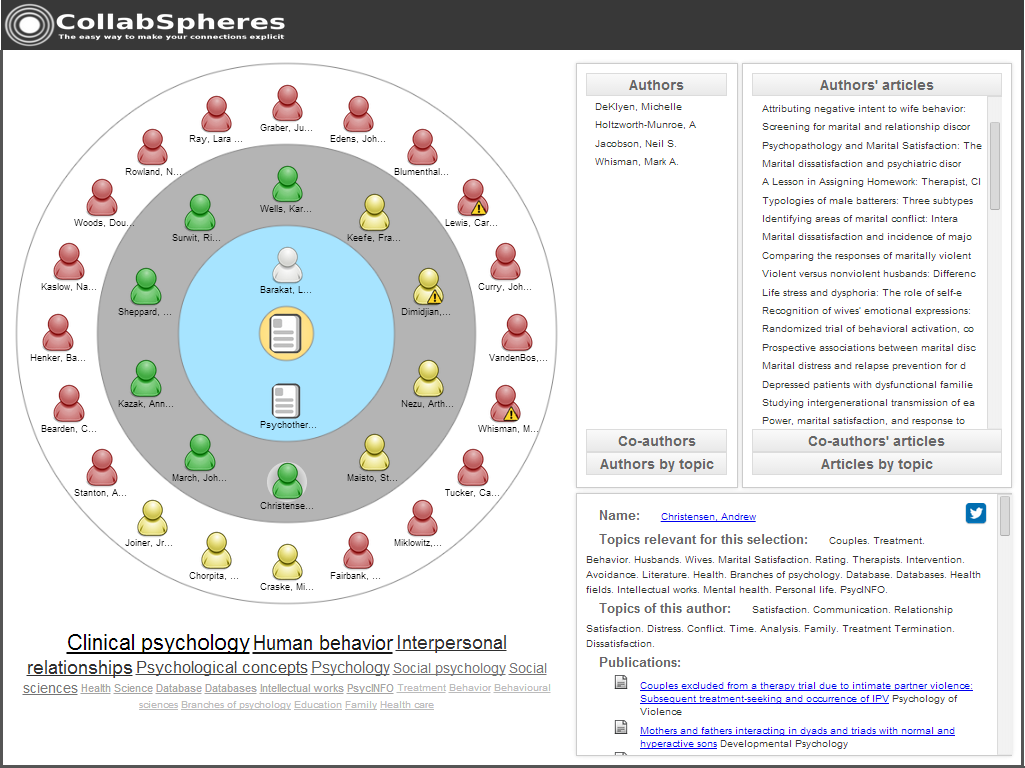
\includegraphics[scale=0.3]{img/CollabAPA.png}
\caption{User interface screenshot}
\label{fig:screenshot}
\end{figure}

%descripción de las acciones y los resultados
%intro
\subsection{Architecture}
The architecture and implementation of the system can be easily divided into three independent modules. Each module provides the needed information to the others creating a complete system.

\begin{description}
  \item[Data Module:] The first module is the data module. The base data used in our scenario is provided by the VIVO APA platform. It consists on an RDF dataset that holds authors and publications that belong to the Psychology domain, together with additional information for each element and the relations between them. One of our tasks related to this dataset has been an information enrichment. Topics form the abstracts and titles have been extracted through NLP techniques and tools for each publication. One of the tools used to perform this task has been TextRazor\footnote{\url{http://www.textrazor.com/} TextRazor provides topic extraction and additional Wikipedia URIs for different categories.} through its API. The second tool that has been used is KT (Knowledge Tagger) working together with a Thesaurus for the psychology domain provided by the APA. Post-processing calculations are used in order to add a weight value for each topic in every article. These topic weights together with the knowledge of the authors that provides the dataset allows the assessment of expertise values for each author. These weighed values are the a key part of data when it comes to recommending experts. The dataset together with the new relations and the added values are stored in a Virtuoso Triplestore. The new dataset offers an explicit representation which allows not only a better understanding of the data but also an improvement when building queries and when retrieving data. The Triplestore is accessible via HTTP SPARQL queries that are posted by the next module:the Web Services.
  \item[Web Services:] The Web Services is in charge of communicating the data form the Data Module to the Front End. It is a web project that triggers different SPARQL queries by using JENA under user request. The results of the queries are processed and returned via REST-JSON web services that respond to the Front End. Some filtering of the data and improvements are done in the Java project, but they are kept as minimum as possible. In this way we try to reduce the impact of this module and use it as a communication channel between the other modules. The power of the Web Services resides on the complex SPARQL queries and the ability to handle user requests.
  \item[Front End] Finally, the Front End Module offers a web application with a browsable interface that is directly available for the users. It has been developed in HTML5, using also javascript, jQuery and CSS. The interface reacts to user actions and throws different Ajax queries to the REST Web Services. Once the JSON response is obtained it is parsed in order to show the results to the users and update the interface as expected. The final result offers a smooth experience that retrieves data through recommendations under user demand.
\end{description}
\begin{figure}[!hbt]
\centering
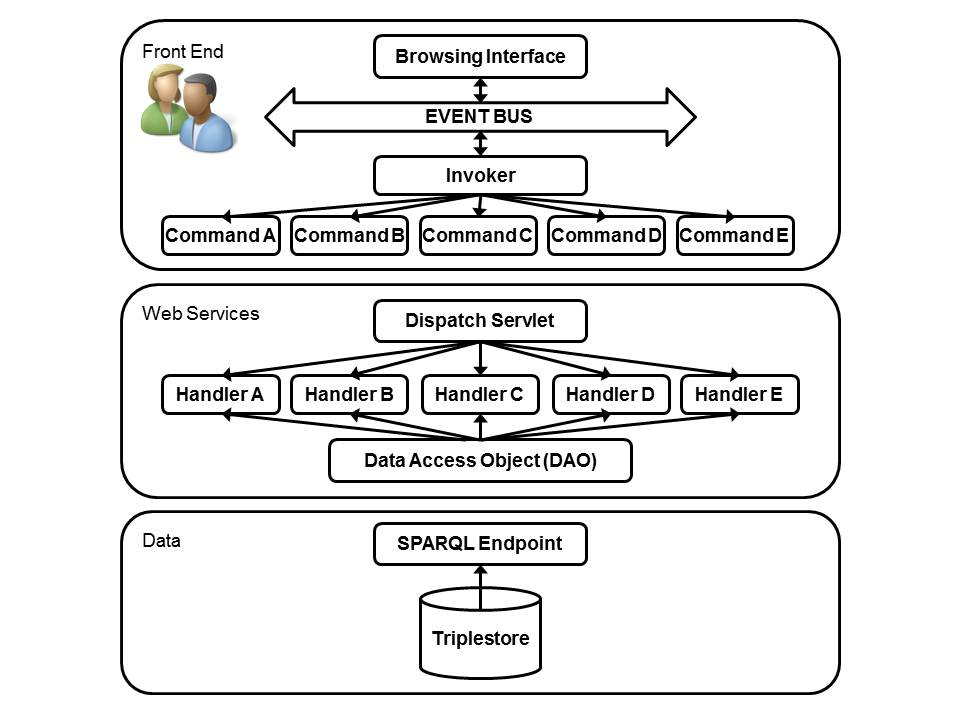
\includegraphics[scale=0.3]{img/APAarchitecture.jpg}
\caption{Basic architecture}
\label{fig:arch}
\end{figure}

